\subsection{Inverse Legueere tessellation}

We compare our implementation with Bourne et all 2026. (Todo: add the 2025 one.)

We have 6 experiment. 
\begin{description}
\item[E1, E2] Bourne et al.'s Voronoi diagram test at $n=20$ and $100$. 
  Bourne2026ConvexOrder, Sec. 6.3.1, Figs. 8-14.
\item[E3, E4] Random power diagrams of our own: random sites \emph{and} varied
  weights. They are irreducible.
\item[E5] Bourne et al.'s cross: generators on the four arms of a plus cut from
  a $40\times40$ lattice, hollow centre, empty corners, all target areas equal.
  It is a reducible power diagram.
  
\item[E6] EBSD image of the steel that showed up for both Bourne 2025 and 2026. Note that this is not a power diagram. Our method returns a power diagram that is closest to the steel image, while Bourne 2026 returns a non-power diagram but with area fitted exactly.
\end{description}

For E1 - E5, reconstructed diargams are shown in figure \ref{} and timing comparsions are recorded in table \ref{}. For E6, we show the reconstructed images in fig \ref{}.


\subsubsection{Running the experiments}

\paragraph*{Running Frank--Wolfe and Subgradient Scheme from Bourne 2026}
Bourne et al.~\cite{Bourne2026} propose two first-order algorithms for recovering generators from prescribed cell areas and barycentres: a Frank--Wolfe method for the projection onto the convex-order set $\mathcal{C}_N$, and a subgradient method for its dual. Both are provided in the notebook accompanying their paper, which we use directly. 
Both start from the paper's second
initial condition $\mathbf{X}_1 = \mathbf{B}_1 = \mathbf{b}$, which puts the generators at the target barycentres and therefore coincides exactly
with our own initialization $\shift = 0$, $\weight = 0$. Both schemes dilate the target to $\lambda\mathbf{b}$ with $\lambda = t/(t-1)$, at the $t$ their paper uses for each instance. We can disable the dilation for the
subgradient scheme but not for Frank--Wolfe, because its generators are recovered as $\mathbf{X} = \lambda\mathbf{b} - \mathbf{B}^\ast$, and a
target read off a real tessellation lies in the achievable set, so at $\lambda = 1$ the projection returns the target itself and every generator collapses to the origin. 
Both method ends with solving a semi-discrete optimal transport problem where the area is enforced, so only their centroid error carries information. 
Empirically \textsc{sg nodil} is the stronger of the two subgradient
variants on every instance, as the dilated form aims
at the fixed point $\mathbf{X} + \mathbf{B}(\mathbf{X}) = \lambda\mathbf{b}$
rather than the true solution.


\paragraph*{Initialization.}
Every method starts from generators placed at the target centroids. For us that
is $\shift=0,\weight=0$, for Borune 2026's methods it is the paper's second
initial condition $\mathbf{Y}_1=\mathbf{B}$. 

\paragraph*{Metric and Reporting}
Every method is measured on the same two quantities, both computed from the
reconstructed diagram: the largest centroid error
$\max_i\|\mathbf{b}_i-\mathbf{c}_i\|$ in domain units, and the largest
relative area error.

Our methods and those of Bourne et al.~\cite{Bourne2026} have different
stopping criteria. For our methods the termination test is applied to the two
gradient blocks, which are precisely the area residual and the area-weighted
entroid residual.
The subgradient scheme stops when its running average stops moving, which the decaying step $\tau_i=2/(i+1)$ guarantees regardless of accuracy, and Frank--Wolfe stops on the duality gap of its own projection problem.
Thus for a fair comparison, we run every method to a fixed budget unless its own test
fires first. The table records how each run ended --- \emph{converged},
\emph{budget} when the iteration cap was reached, or \emph{stalled} when the
line search failed --- together with the iteration at which it stopped and the
time taken to reach the error reported.

Wall-clock seconds are reported, with the caveat that our implementations are
compiled C\texttt{++} while FW and SG are Python driving \texttt{pysdot},
whose core is itself C\texttt{++}. This contributes a constant factor to the
timing gaps.
 


%%%%%%%%%%%%%%%%%%%%%%%%%%%%%%%%%%%%%%%%%%%%%%%%%%
%%%%%%%%%% comparison table %%%%%%%%%%%%%%%%%%%%%%
%%%%%%%%%%%%%%%%%%%%%%%%%%%%%%%%%%%%%%%%%%%%%%%

\begin{table}[h]
\centering \small
\setlength{\tabcolsep}{3pt}
\caption{E1 - E5 using five methods.
The outcome column gives how each run
  ended and, in parentheses, the iteration at which it did: \emph{converged}
  on the method's own test, \emph{stalled} on a line-search failure, or
  \emph{budget} on the iteration cap. Iteration counts are not comparable
  across methods, so we measure the runtime.``area error'' measures the largest relative area error and
  ``centorid error'' is $\max_i\|\mathbf{b}_i-\mathbf{c}_i\|$, both measured on the
  diagram each method holds when it stops. We dilated FW and SG dil with $t=1250$ for E1--E4
  and $t=100$ for E5, consistent with the setting in their paper.}
\label{tab:results}
\begin{tabular}{llrrr}
\toprule
method & outcome (iters) & runtime(s) & area error & centroid error \\
\midrule
\multicolumn{5}{l}{\textbf{E1}\; Bourne et al.\ Voronoi, $n=20$}\\[1pt]
Block Ascend & budget {\scriptsize (5000)} & 3.25 & 1.3e-14 & 7.0e-9 \\
Joint Newton & converged {\scriptsize (357)} & 0.05 & 4.2e-12 & 6.6e-11 \\
FW & budget {\scriptsize (2001)} & 24.40 & 2.0e-7 & 7.2e-5 \\
SG dil & budget {\scriptsize (2000)} & 27.45 & 2.0e-7 & 7.5e-5 \\
SG nodil & budget {\scriptsize (2000)} & 10.28 & 1.4e-6 & 1.2e-3 \\
\midrule
\multicolumn{5}{l}{\textbf{E2}\; Bourne et al.\ Voronoi, $n=100$}\\[1pt]
Block Ascend & stalled {\scriptsize (59)} & 0.11 & 2.4e-8 & 2.9e-4 \\
Joint Newton & converged {\scriptsize (2014)} & 1.08 & 1.4e-11 & 2.5e-10 \\
FW & budget {\scriptsize (2001)} & 33.15 & 2.6e-6 & 7.6e-4 \\
SG dil & budget {\scriptsize (2000)} & 41.41 & 4.0e-5 & 2.0e-2 \\
SG nodil & budget {\scriptsize (2000)} & 13.66 & 4.0e-6 & 8.7e-4 \\
\midrule
\multicolumn{5}{l}{\textbf{E3}\; Random power diagram, $n=20$}\\[1pt]
Block Ascend & budget {\scriptsize (5000)} & 10.20 & 6.5e-8 & 1.6e-7 \\
Joint Newton & converged {\scriptsize (419)} & 0.06 & 6.9e-11 & 5.7e-10 \\
FW & converged {\scriptsize (1522)} & 17.05 & 1.7e-11 & 9.9e-5 \\
SG dil & budget {\scriptsize (2000)} & 43.62 & 2.7e-11 & 3.8e-2 \\
SG nodil & budget {\scriptsize (2000)} & 13.79 & 2.8e-10 & 2.7e-3 \\
\midrule
\multicolumn{5}{l}{\textbf{E4}\; Random power diagram, $n=100$}\\[1pt]
Block Ascend & stalled {\scriptsize (883)} & 2.36 & 9.6e-7 & 1.1e-1 \\
Joint Newton & budget {\scriptsize (5000)} & 3.11 & 1.0e-7 & 2.1e-5 \\
FW & budget {\scriptsize (2001)} & 45.14 & 6.1e-3 & 3.9e-3 \\
SG dil & budget {\scriptsize (2000)} & 75.94 & 3.2e-3 & 2.6e-2 \\
SG nodil & budget {\scriptsize (2000)} & 21.16 & 1.1e-6 & 2.5e-3 \\
\midrule
\multicolumn{5}{l}{\textbf{E5}\; Bourne et al.\ reducible, $N=728$}\\[1pt]
Block Ascend & stalled {\scriptsize (49)} & 3.99 & 3.2e-4 & 1.9e-3 \\
Joint Newton & stalled {\scriptsize (23)} & 0.23 & 6.9e-4 & 2.4e-3 \\
FW & budget {\scriptsize (1501)} & 68.94 & 1.1e-8 & 1.8e-2 \\
SG dil & budget {\scriptsize (1500)} & 57.83 & 1.1e-8 & 1.8e-2 \\
SG nodil & budget {\scriptsize (1500)} & 31.59 & 1.2e-7 & 1.5e-2 \\
\bottomrule
\end{tabular}
\end{table}



\begin{figure*}[p]
\centering
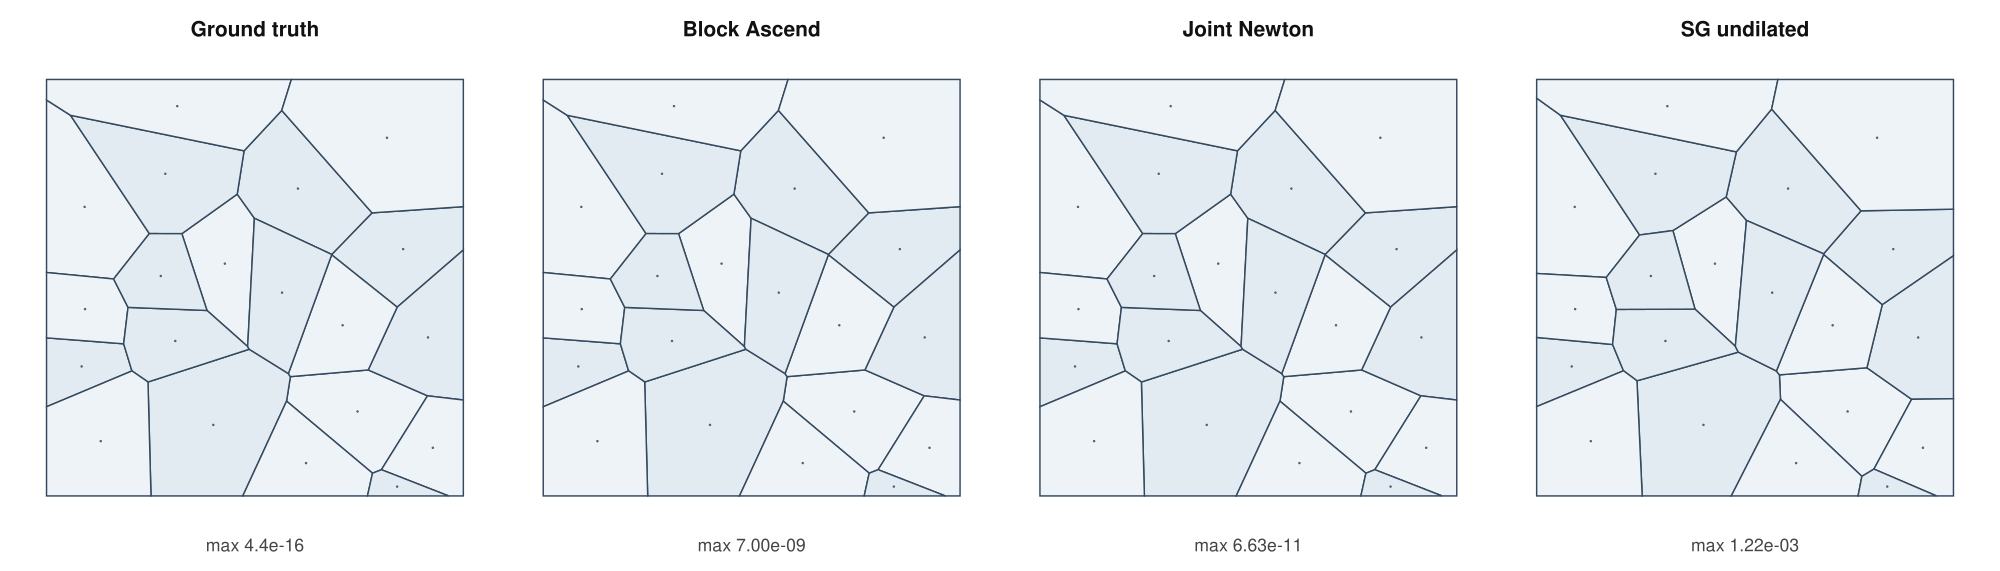
\includegraphics[width=0.84\linewidth]{inversetessellations/fig/row_pd_bourne_voronoi_n20.png}\\[2pt]
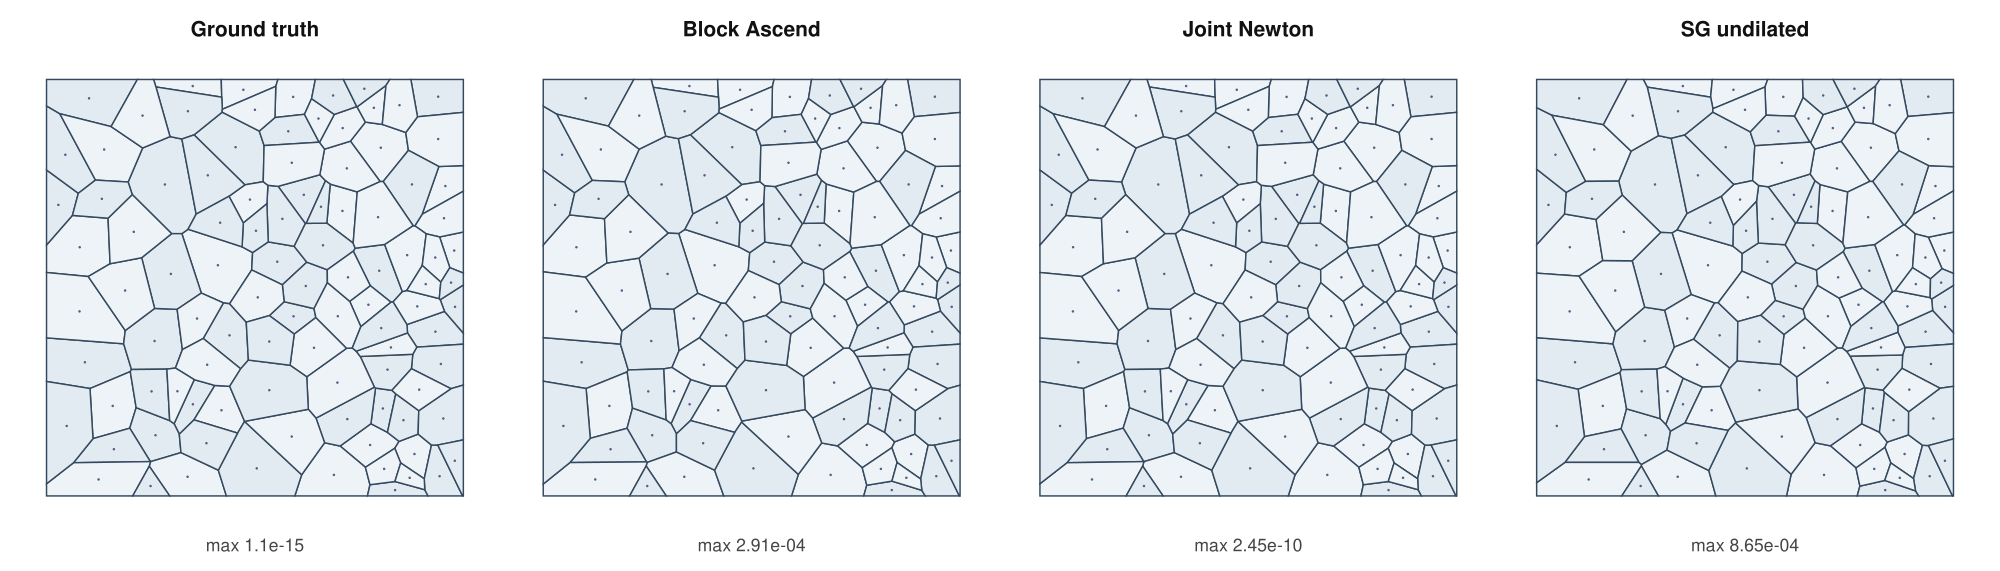
\includegraphics[width=0.84\linewidth]{inversetessellations/fig/row_pd_bourne_voronoi_n100.png}\\[2pt]
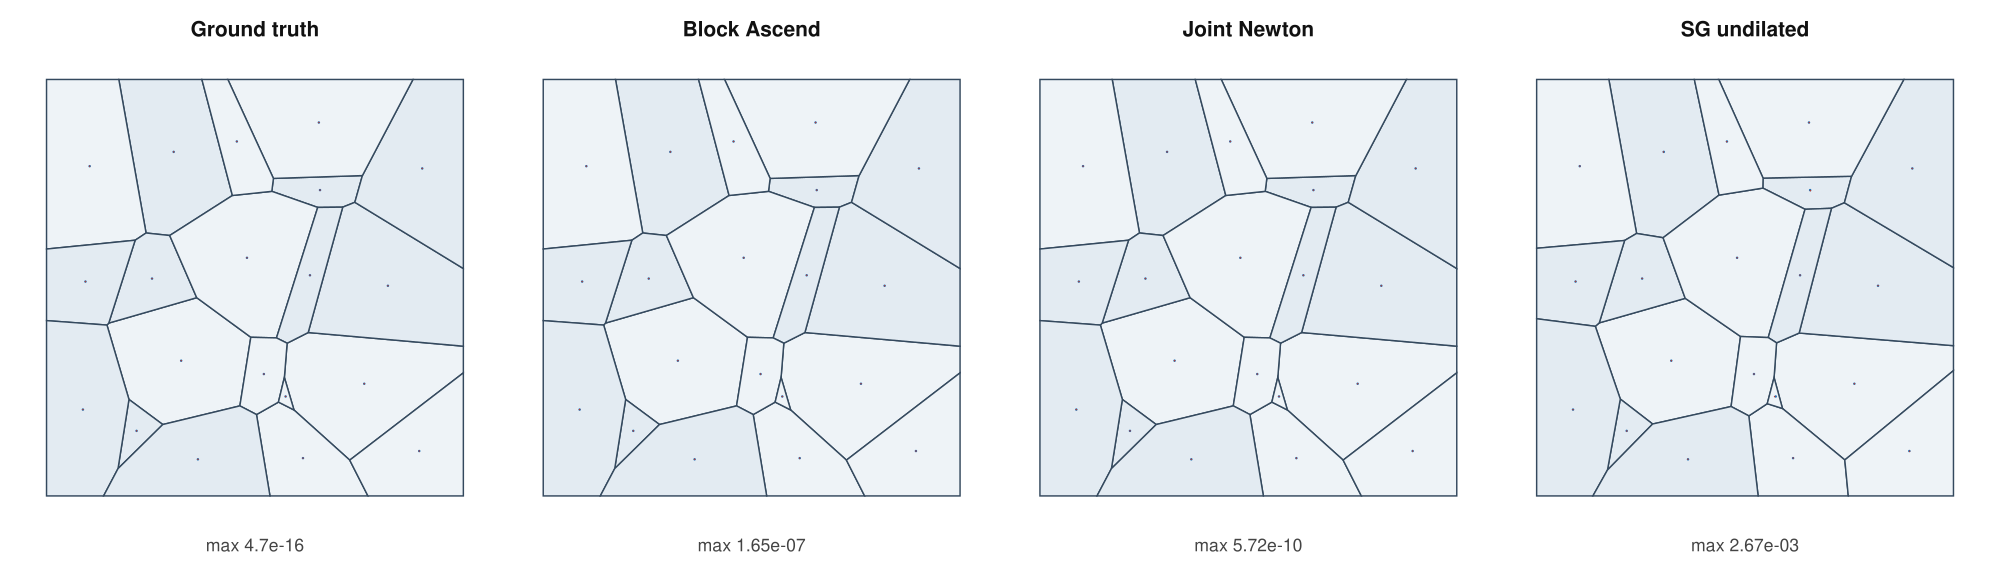
\includegraphics[width=0.84\linewidth]{inversetessellations/fig/row_pd_random_power_n20.png}
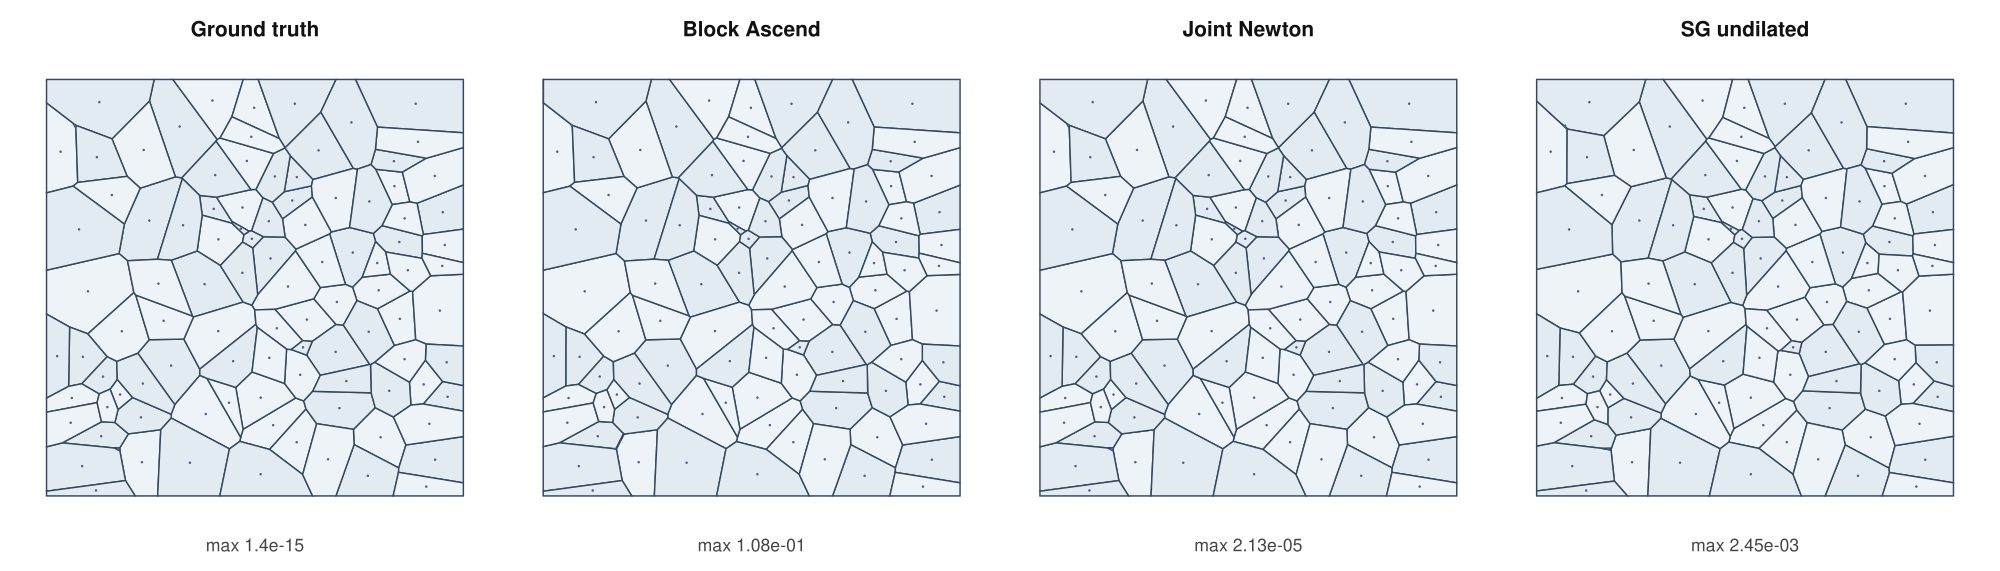
\includegraphics[width=0.84\linewidth]{inversetessellations/fig/row_pd_random_power_n100.png}\\[8pt]
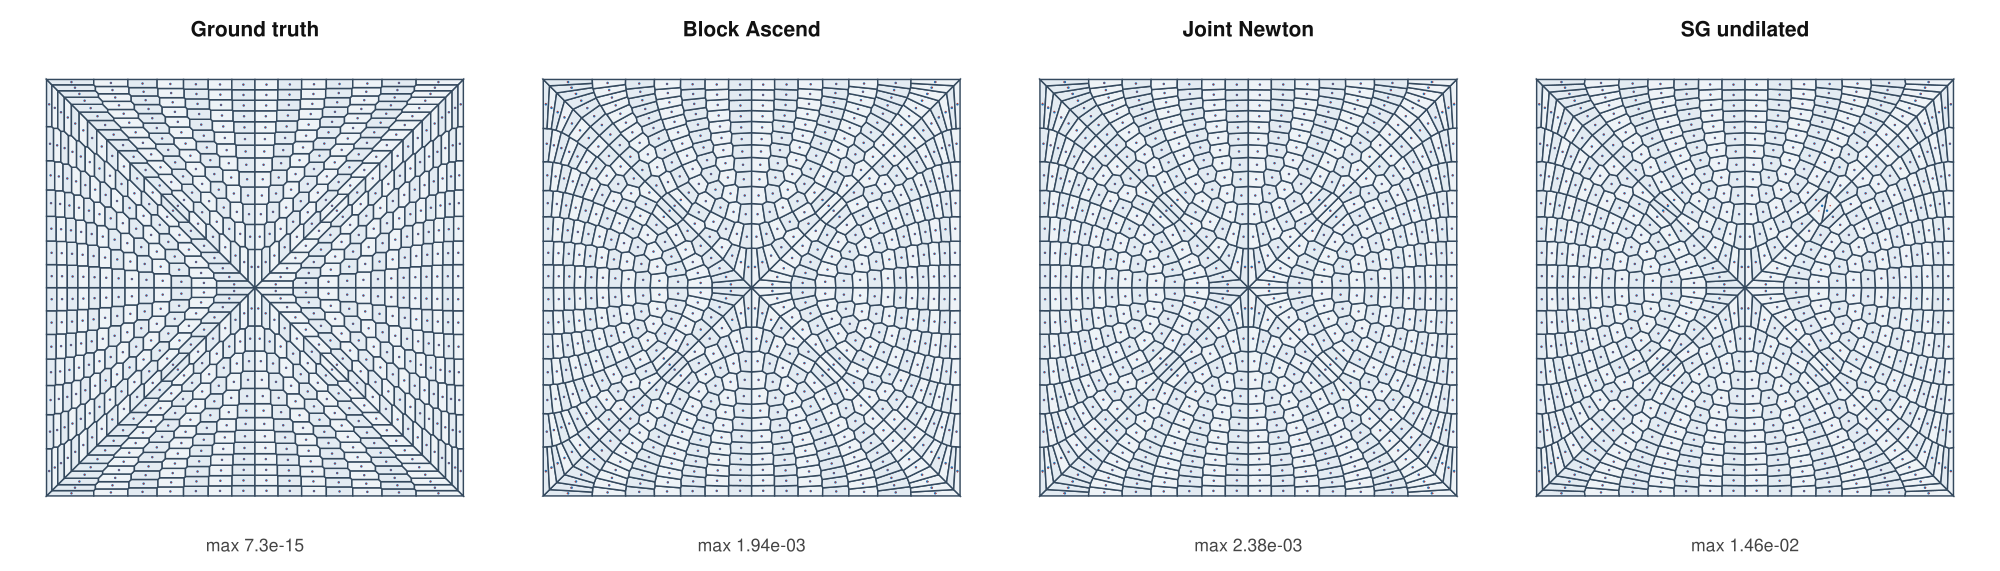
\includegraphics[width=0.84\linewidth]{inversetessellations/fig/row_pd_bourne_cross_n728.png}
\caption{E1 (top), E2 (middle), E3 (bottom). Blue dots are the target
  barycentres $\mathbf{b}_i$, red the achieved centroids $\mathbf{c}_i$; where a
  cell is fitted the two coincide. All four panels of a row are drawn by the
  same renderer from the same instance, so any difference is in the
  tessellation, not in the drawing.
  E4 (top) and E5 (bottom). In E4 \textsc{Block Ascend}'s tessellation is visibly
  wrong --- it stalls at $1.1\cdot10^{-1}$ --- while \textsc{Joint Newton} is
  indistinguishable from the truth. In E5 \emph{no} method recovers the
  herringbone of the ground truth, and \textsc{Joint Newton} and \textsc{sg}
  converge to visibly the same incorrect tessellation from completely different
  directions.}
\label{fig:rows1}
\end{figure*}


\subsubsection{Reading the results}

\paragraph*{Discussions on our methods.} 
Our Joint Newton methods generally out peforms the rest.
On E1--E4 it reaches $6.6\cdot10^{-11}$, $2.5\cdot10^{-10}$,
$5.7\cdot10^{-10}$ and $2.1\cdot10^{-5}$, three to six orders of magnitude
below schemes from Bourne2026. It takes $0.05$ to $3.1$ seconds where they
take $10$ to $76$. The gap is too large to be simply be an artifact of
C\texttt{++} against Python. 
Meanwhile, our Block Ascend stalls.
It fails on three of five instances: E2 at $2.9\cdot10^{-4}$ after $59$
iterations, E4 at $1.1\cdot10^{-1}$ after $883$, and E5 at $1.9\cdot10^{-3}$
after $49$. In each the line search cannot find a step that lowers the
residual, and the solver stops far from convergence.
Where Block Ascend does reach high accuracy, on E1 and E3, it uses the whole budget and is $65$ to $170$ times slower than
Joint Newton.

\paragraph*{Discussions on Bourne2026's methods}
The subgradient scheme
can be undilated, which is worth between $1.2$ and $23$ times on E2--E5,
since the dilated form aims at
$\mathbf{X}+\mathbf{B}(\mathbf{X})=\lambda\mathbf{b}$ rather than
$\mathbf{B}(\mathbf{X})=\mathbf{b}$. 





\paragraph*{All methods fail on E5.}
All five land between $1.9\cdot10^{-3}$ and $1.8\cdot10^{-2}$, against a
reachable $7.3\cdot10^{-15}$, and Figure~\ref{fig:rows2} shows ours and
theirs settling on visibly the same incorrect tessellation. 

\begin{figure*}[t]
\centering
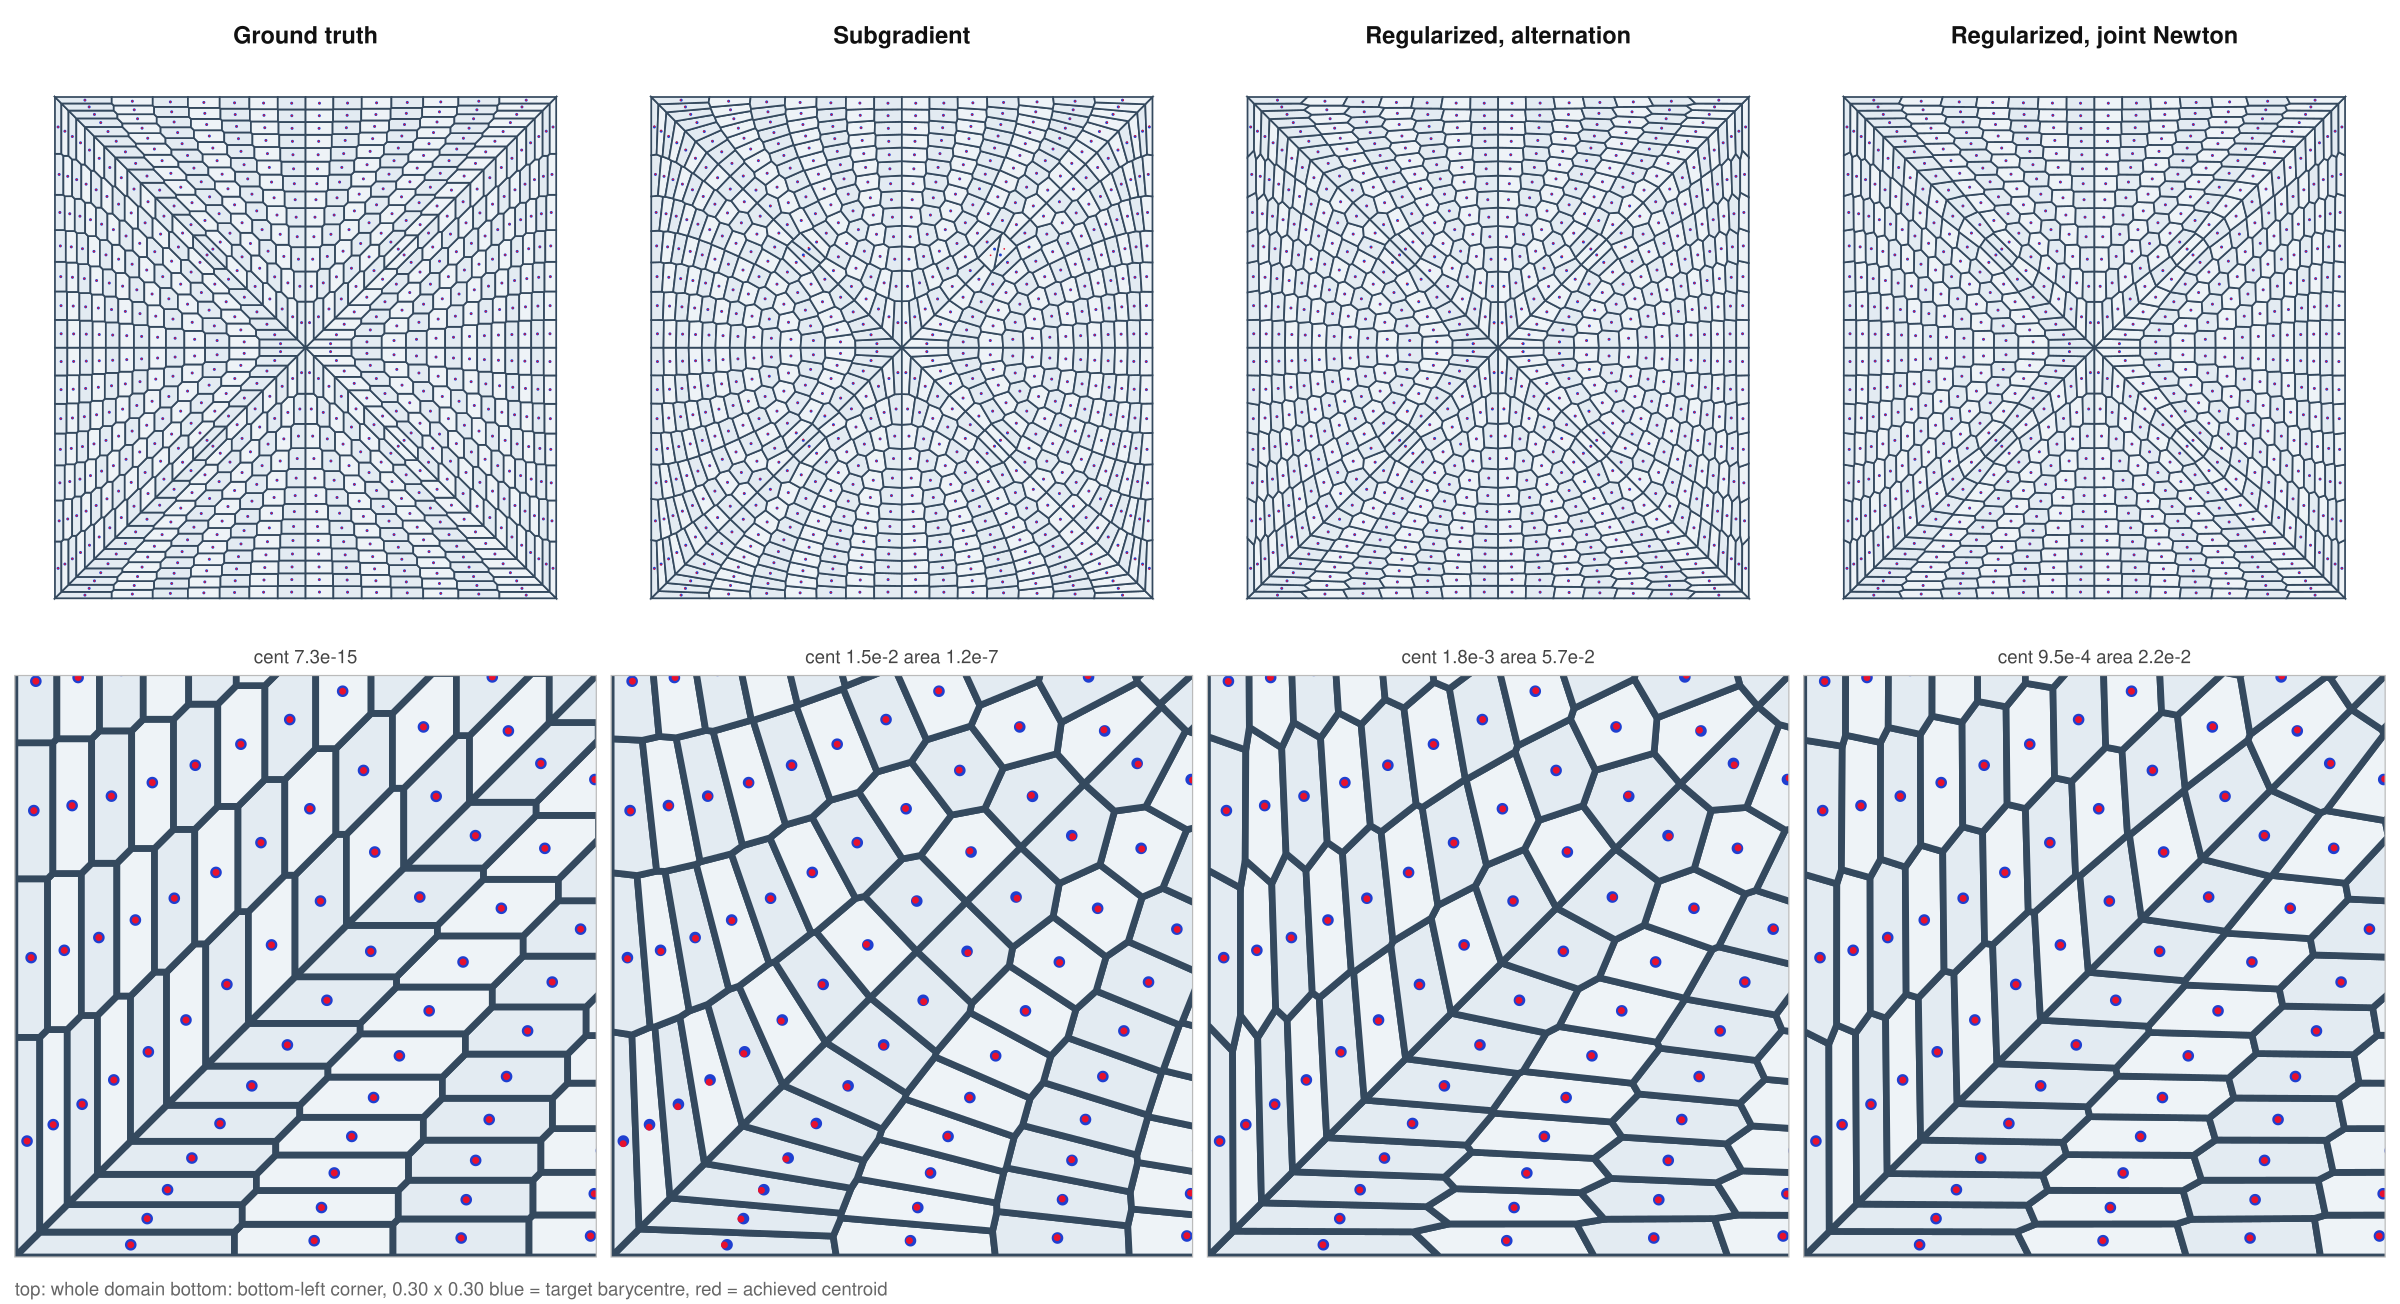
\includegraphics[width=0.92\linewidth]{inversetessellations/fig/row_final_cross.png}
\caption{Figure N. Fitting the reducible $N=728$ cross of Bourne et al. Top: the whole domain; bottom: the bottom-left corner, $0.30\times0.30$. Blue dots are the target barycentres $\mathbf{b}_i$, red the achieved centroids. The ground-truth tessellation is a herringbone — two families of long thin cells meeting along a straight diagonal seam running from each corner to the centre. The subgradient scheme of Bourne et al. and the regularized solve under its shipped alternation both return a rounded radial fan that loses this structure entirely, differing from each other mainly in where the error is concentrated: the subgradient scheme meets the cell areas by construction, since every iterate is recovered through a transport solve, while the alternation surrenders $5.7\%$ of area error. Solving the same entropic problem with a joint Newton step over $(\mathbf{s}, \mathbf{z}, \mathbf{u})$ instead of alternating between the grid and point blocks recovers the herringbone, and attains the lowest centroid error of any method we tested on this instance, $9.5\cdot10^{-4}$. The regularization is $\varepsilon = 3\cdot10^{-4}$ on a $256^2$ grid for both regularized columns; the joint solve reaches its result in $45$ iterations and $71$ seconds, against $176$ seconds and $4000$ iterations for the alternation, which never drives both marginals down together — forcing either one to $10^{-15}$ leaves the other near $10^{-2}$.}
\label{fig:ebsd}
\end{figure*}

\begin{figure*}[t]
\centering
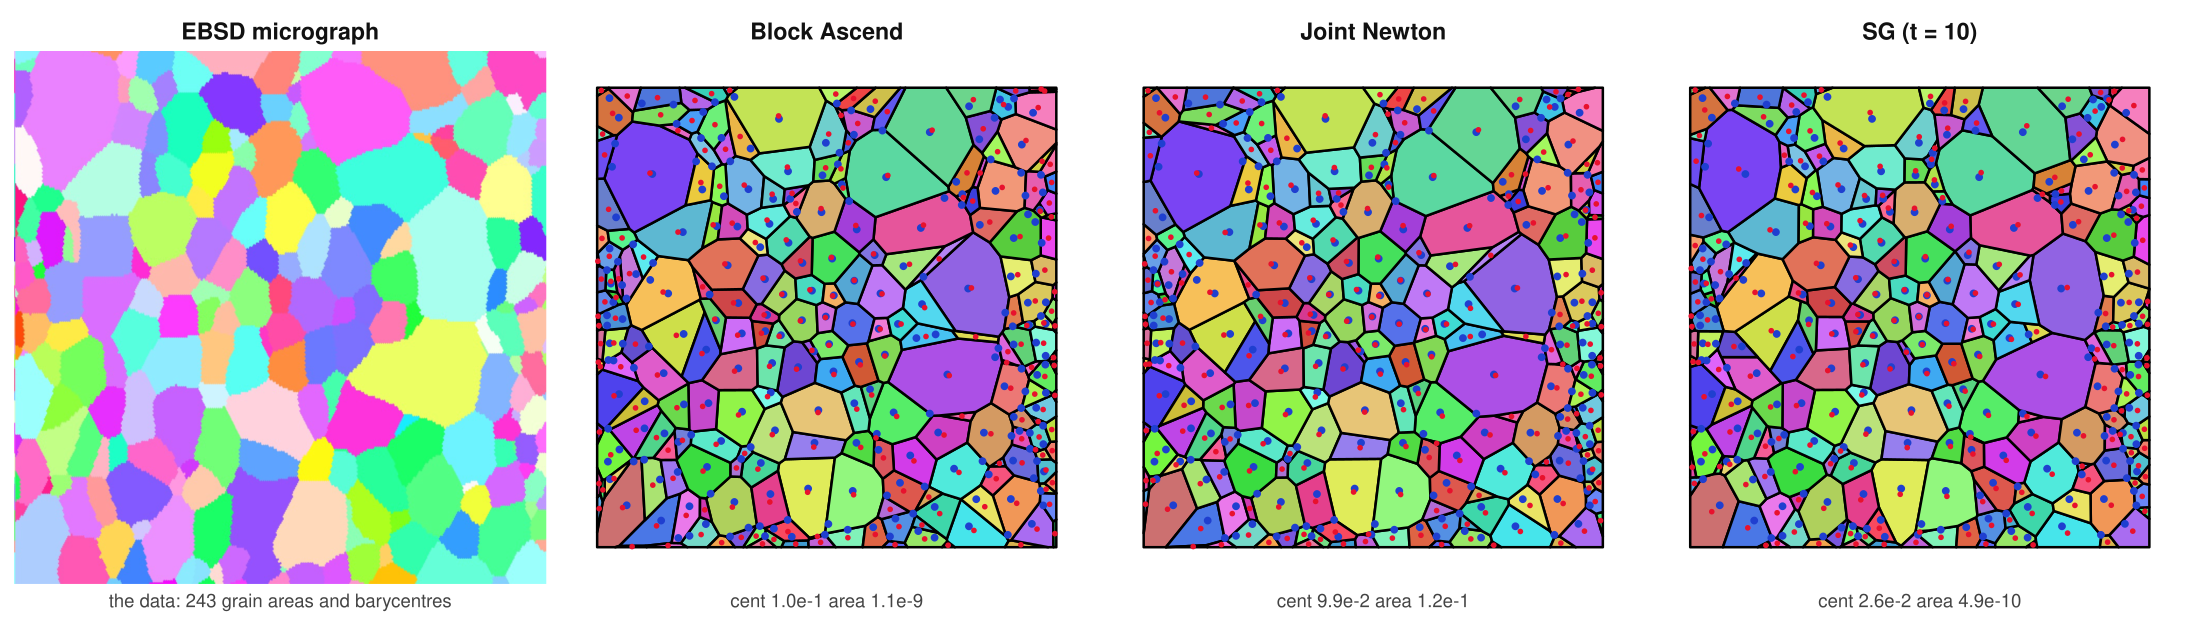
\includegraphics[width=0.92\linewidth]{inversetessellations/fig/row_ebsd.png}
\caption{The EBSD steel micrograph of Bourne et al.\ \cite{Bourne2026},
  $N=243$ grains, with the areas and barycentres of those grains as the
  targets. This is not a valid diagram, so ours doesn't converge. Might be a good idea to run the one with softened constraints.}
\label{fig:ebsd}
\end{figure*}